
\section{Konvolučné neurónové siete}
\label{sec:architekuraCNN}

\subsection{Nastavenie parametrov}
\label{subsec:nastavenieparametrov}
Ako bolo spomínané v kapitole \ref{subsec:convolutionalneuralnetwork} je niekoľko parametrov, ktoré je potrebné
    nastaviť v konvolučných a pooling vrstvách.
Pre správne fungovanie sietíe je potrebné nastaviť aj správne hodnoty týchto parametrov, preto v navrhovaných architektúrach budú
    hodnoty parametrov nastavené na tie najpoužívanejšie.

Veľkosť výstupu a správnosť nastavenia parametrov v konvolučnej vrstve je možné výpočítať pomocou vzťahu:
\begin{equation}
    \frac{(W - F + 2*P)}{S} + 1
\end{equation}
Kde $W$ je veľkosť vstupných dát, $F$ je veľkosť filtra, $P$ je nastavenie zarovnania, v prípade nulového zarovnania je hodnota 1 a $S$ je veľkosť kroku.
Pre správne nastavenie musí byť výsledná hodnota celé číslo, kde táto výsledná hodnota udáva aj veľkosť výstupu.
Najpoužívanejšie hodnoty parametrov sú: $F = 3, S = 1, P = 1$ a vstup $W$ o hodnote, ktorá je deliteľná číslom 2 \cite{odkaz:CNNArchitecture}.

Funkciou pooling vrstvy je znižovanie dimenzionality a zároveň ponechanie dôležítých informácií, ako najpoužívanejšie hodnoty parametrov sú
    veľkosť filtra 2x2 s krokom 2 pri použití MaxPooling vrstvy \cite{odkaz:CNNArchitecture}.

% TODO batch-size, epochy
% CNN sa trenuje v cykloch nazyvanych epochy, v kazdej epoche prejdu cez sieť vsetky obrazky na ktorych sa sieť uci,
% pre ucenie je potrebne zvolit vhodny pocet tychro epoch aby sieť podala najelpsie vysledky a zaroven sa nepretrenovala.
% Preto je vhodne ukoncit trenovanie v bode kedy klesa presnost siete na validacnych datach, v takom pripade to moze vies k pretrénovaniu siete
% na trenovacich datach.

\subsection{Návrh architektúr}
\label{subsec:navrharchitektur}
Prvý model siete je inšpirovaný architektúrou AlexNet (viď. \ref{subsec:popularCNN}).
Model obsahuje celkovo 20 vrstiev, z ktorých 5 je konvolučných, 5 max pooling, 7 dropout a 3 dense vrstvy.
Veľkosť vstupných dát do prvej vrstvy je 128x128x3.
Vo všetkých konvolučných vrstvách sú použité filtre o veľkosti 3x3 s krokom 1 a použitím nulové zarovnania.

V modeli sa každou konvolučnou vrstvou zdvojnásobuje počet filtrov, s počiatočných 16 až na 256 v poslednej vrstve.
Pooling vrstvy sú typu max, veľkosť filtra je 2x2 s posunom 2 po každej osi.
Za každou pooling vrstvou sa nachádza Droupout vrstva s nastavením 0.2, ciže 20 percent náhodných prepojení sa ignoruje.

Po piatich blokoch konvolučnej, pooling a droupout vrstvy nasledujú 2 dense vrstvy s počtom prepojení 1024 a dropout vrstvou s nastavním 0.5.
Ako posledná je dense vrstva s 2 alebo 72 prepojeniami a softmax klasifikátorom, počet výstupov záleží, či určujeme typ alebo náklon zbrane.
V celej sietí sú použité ReLu aktivačné funkcie.

\begin{figure}[H]
    \centering
    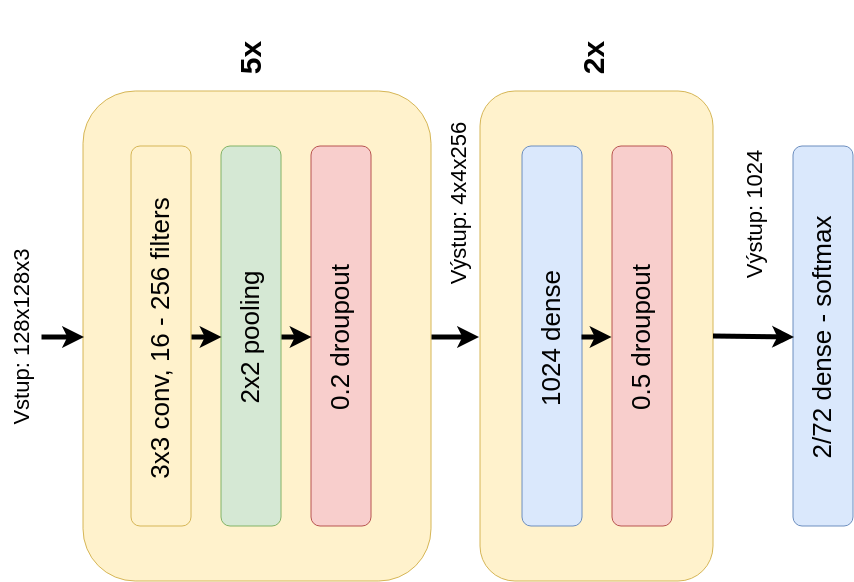
\includegraphics[width=0.6\textwidth]{AlexNet_Like}
    \caption{AlexNet-Like navrhovaná architektúra.}
    \label{pic:kNN}
\end{figure}

% ----------- DRUHY NAVRH -----------

Druhý navrhovaný model je inšpirovaný architektúrou VGG sietí (viď. \ref{subsec:popularCNN}).
Vzhľadom na možnosti výkonu na ktorom bude trénovanie prebiehať, je navrhovaná sieť o dva bloky vrstviev menšia a taktiež konvolučne vrstvy obsahujú menej filtrov.

Celkovo sieť obsahuje 2 bloky obsahujúce 2 konvolučné vrstvy s počtom filtrov 32 a 64, pooling a droupout vrstvu s 20\% ignorovaním prepojení.
Ďalej nasledujú 3 konvolučné vrstvy so 128 filtrami a pooling vrstva.
Ako posledné sú 2 bloky obsahujúce dense vrstvu s počtom prepojení 2048 a dropout vrstvu s ignorovaním nastaveným na 50\%.
Posledná výstupná vrstva obsahuje 2 alebo 72 prepojení so softmax klasfikátorom.
Každá konvolučna vrstva obsahuje filtre o veľkosti 3x3, krokom 1 a s použitím nulového doplnku.
Pooling vrstvy sú typu max, veľkosť filtra je 2x2 s posunom 2 po každej osi.
V celej sietí je použitá ReLu aktivačná funkcia.

\begin{figure}[H]
    \centering
    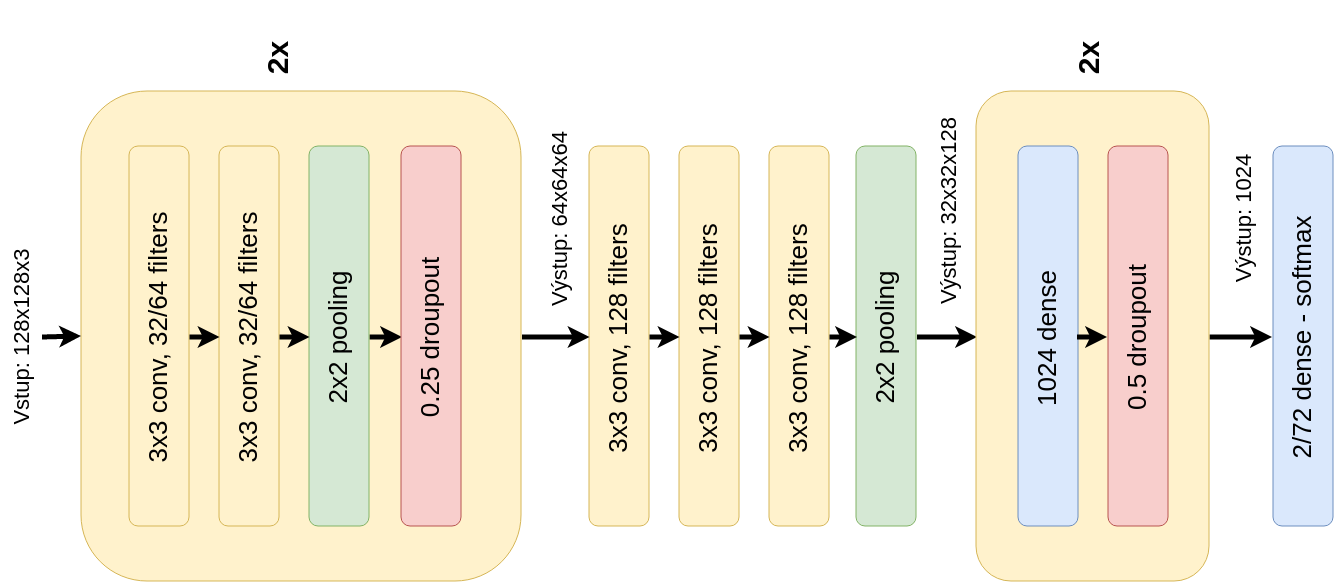
\includegraphics[width=0.8\textwidth]{VGG_Like}
    \caption{VGG-Like navrhovaná architektúra.}
    \label{pic:kNN}
\end{figure}
